
\documentclass[conference]{IEEEtran}

\usepackage{cite}
\usepackage{amsmath,amssymb,amsfonts}
\usepackage{algorithmic}
\usepackage{graphicx}
\usepackage{textcomp}
\usepackage{bm}
\usepackage{upgreek}

%\usepackage[retainorgcmds]{IEEEtrantools}

\usepackage{hyperref}

\usepackage[nottoc]{tocbibind}


%\linespread{1.3}


\title{Predictive Distribution Estimation for Bayesian Machine Learning using a Dirichlet Prior}

\author{
\IEEEauthorblockN{Paul Rademacher}
\IEEEauthorblockA{U.S. Naval Research Laboratory\\Radar Division\\Washington, DC 20375, USA}
\and
\IEEEauthorblockN{Milo\v{s} Doroslova\v{c}ki}
\IEEEauthorblockA{The George Washington University\\Department of Electrical and Computer Engineering\\Washington, DC 20052, USA}
}


%\graphicspath{ {C:/Users/Paul/Documents/PhD/Dissertation/Documentation/Figures/} }
\graphicspath{ {../Figures/} }


\DeclareMathOperator*{\argmin}{arg\,min}
\DeclareMathOperator*{\argmax}{arg\,max}

\DeclareMathOperator{\xrm}{\mathrm{x}}
\DeclareMathOperator{\Xrm}{\mathrm{X}}
\DeclareMathOperator{\yrm}{\mathrm{y}}
\DeclareMathOperator{\Yrm}{\mathrm{Y}}
\DeclareMathOperator{\Drm}{\mathrm{D}}
\DeclareMathOperator{\nrm}{\mathrm{n}}
\DeclareMathOperator{\nbarrm}{\bar{\mathrm{n}}}
\DeclareMathOperator{\zrm}{\mathrm{z}}

\DeclareMathOperator{\Prm}{\mathrm{P}}
\DeclareMathOperator{\prm}{\mathrm{p}}
\DeclareMathOperator{\Erm}{\mathrm{E}}
\DeclareMathOperator{\Crm}{\mathrm{C}}

\DeclareMathOperator{\Xcal}{\mathcal{X}}
\DeclareMathOperator{\Ycal}{\mathcal{Y}}
\DeclareMathOperator{\Dcal}{\mathcal{D}}
\DeclareMathOperator{\Ncal}{\mathcal{N}}
\DeclareMathOperator{\Zcal}{\mathcal{Z}}
\DeclareMathOperator{\Hcal}{\mathcal{H}}
\DeclareMathOperator{\Fcal}{\mathcal{F}}
\DeclareMathOperator{\Rcal}{\mathcal{R}}
\DeclareMathOperator{\Mcal}{\mathcal{M}}
\DeclareMathOperator{\Scal}{\mathcal{S}}
\DeclareMathOperator{\Pcal}{\mathcal{P}}

\DeclareMathOperator{\Rbb}{\mathbb{R}}
\DeclareMathOperator{\Nbb}{\mathbb{N}}
\DeclareMathOperator{\Zbb}{\mathbb{Z}}

\DeclareMathOperator{\Dir}{\mathrm{Dir}}
\DeclareMathOperator{\DM}{\mathrm{DM}}
\DeclareMathOperator{\Mult}{\mathrm{Mult}}
\DeclareMathOperator{\DP}{\mathrm{DP}}









\begin{document}

\maketitle

% As a general rule, do not put math, special symbols or citations
% in the abstract
\begin{abstract}
In Bayesian treatments of machine learning, the success or failure of the estimator/classifier hinges on how well the prior distribution selected by the designer matches the actual data-generating model. This paper assumes that the data-generating PMF is a realization of a Dirichlet process and assesses the mismatch between the true predictive distribution and the predictive distribution approximated using the training data. It is shown that highly localized Dirichlet priors can overcome the burden of a limited training set when the prior mean is well matched to the true distribution, but will degrade the approximation if the match is poor. A bias/variance tradeoff will be demonstrated with illustrative examples.
\end{abstract}


\section{Introduction}

PGR: make changes from Extended Summary...

This article investigates how a Bayesian perspective influences the predictive distributions used to make decisions in machine learning applications. The efficacy of Bayesian learning methods depends on how well the prior knowledge imparted by the designer matches reality. The chosen prior distribution over the set of data-generating probability mass functions (PMF) reflects the users confidence that different PMF's are responsible for generating the observed/unobserved random elements. If a highly subjective prior is chosen that strongly weights the actual data PMF, low risk learning functions are possible even with limited training data; however, if the prior is poorly selected, a good solution will never be achieved. Conversely, a non-informative prior that treats the different PMF's will always be able to adapt will enough training data; if data is limited, however, the learning function may not deliver the required performance.

This work assumes that the prior distribution is Dirichlet. The class of Dirichlet probability density functions (PDF) have the desirable properties of full support over the set of possible PMF's and a tractable posterior distribution for independently and identically distributed data \cite{ferguson}. The full support is necessary to ensure that the true underlying model can be identified with enough training data. Also, control of the Dirichlet parameters can enable both objective and subjective prior distributions. 

Once the Bayesian assumption is used to form the predictive distribution conditioned on the training data, it will be compared to the true predictive distribution given knowledge of the model PMF. Specifically, the first and second joint moments of the difference between the two PMF's will be determined. Specific attention will be given to various asymptotic cases of the Dirichlet distribution to illustrate the bias/variance tradeoff for both uninformative and subjective priors.







\section{Objective}

Consider an observable discrete random element $\xrm \in \Xcal$ and and unobservable discrete random element $\yrm \in \Ycal$ which are jointly distributed according to an unknown PMF $\uptheta \in \Theta = \Pcal(\Ycal \times \Xcal)$, where $\Pcal(\cdot)$ denotes the full space of PMF's over the argument set. As such, $\Prm_{\yrm,\xrm | \uptheta}(y,x) = \uptheta(y,x)$. Also observed is a random sequence of $N$ samples from $\uptheta$, denoted $\Drm = ( \Yrm,\Xrm ) \in \Dcal = \{\Ycal \times \Xcal\}^N$. The $N$ data pairs are conditionally independent from one another and are identically distributed as $\Prm_{\Drm_n | \uptheta}(y,x) = \uptheta(y,x)$. The samples are also conditionally independent from $(\yrm,\xrm)$. Thus,
\begin{equation}
\Prm(\yrm,\xrm,\Drm | \uptheta) = \Prm(\yrm,\xrm | \uptheta) \prod_{n=1}^N \Prm\big( \Drm_n | \uptheta \big) \;.
\end{equation}

The metric guiding the design is a loss function $\mathcal{L}: \Hcal \times \Ycal \mapsto \Rbb_{\geq 0}$ which penalizes the decision $h \in \Hcal$ based on the value of $\yrm$. Define the conditional expected loss, or conditional ``risk'',
\begin{equation} \label{eq:risk_cond}
\Rcal_{\Theta}(h ; \uptheta) = \Erm_{\Drm | \uptheta} \bigg[ \Erm_{\yrm,\xrm | \uptheta} \Big[ \mathcal{L}\big( h,\yrm \big) \Big] \bigg] \;.
\end{equation}


If the model $\uptheta$ were known, for a given set of observations a ``clairvoyant'' decision $h = \argmin_{h \in \Hcal} \Erm_{\yrm | \xrm,\Drm,\uptheta}\big[ \mathcal{L}(h,\yrm) \big]$ could be made to minimize this objective. It can be shown that given the model $\uptheta$, the unobserved element $\yrm$ is conditionally independent of the training data $\Drm$. As such, the knowledge of $\uptheta$ renders $\Drm$ uninformative and the clairvoyant decision depends on the true predictive distribution $\Prm(\yrm | \xrm,\uptheta)$.


However, as the model $\uptheta$ is not observed, this predictive PMF is unknown and the conditional risk is not yet a valid objective function for optimization. To remove the dependency on $\uptheta$, the model is treated as a random process and a Bayesian approach is adopted. The Bayes risk can be formulated as
\begin{IEEEeqnarray}{rCl} \label{eq:risk}
\Rcal(h) & = & \Erm_{\uptheta}\big[ \Rcal_{\Theta}(h ; \uptheta) \big] \\
& = & \Erm_{\xrm,\Drm}\Big[ \Erm_{\yrm | \xrm,\Drm} \big[ \mathcal{L}(h,\yrm) \big] \Big] \nonumber
\end{IEEEeqnarray}
and $\yrm$, $\xrm$, and $\Drm$ are treated as jointly distributed random elements.

For a given set of observations, the optimal Bayesian decision is $h = \argmin_{h \in \Hcal} \Erm_{\yrm | \xrm,\Drm}\big[ \mathcal{L}(h,\yrm) \big]$, dependent on the conditional PMF $\Prm(\yrm | \xrm,\Drm)$. This conditional predictive distribution can be interpreted as an estimate of the true predictive distribution $\Prm(\yrm | \xrm,\uptheta)$.












\section{Probability Distributions}

This section introduces the Dirichlet prior distribution for the model $\uptheta$ and uses it to formulate the estimated predictive distribution $\Prm(\yrm | \xrm,\Drm)$.


\subsection{Model PDF, $\prm(\uptheta)$} \label{sec:P_theta}

The Dirichlet PDF for the model $\uptheta \in \Theta$ is \cite{bishop}
\begin{IEEEeqnarray}{rCl}
\prm(\uptheta) & = & \beta(\alpha)^{-1} \prod_{y \in \Ycal} \prod_{x \in \Xcal} \uptheta(y,x)^{\alpha(y,x) - 1} \;,
\end{IEEEeqnarray}
where the user-selected PDF parameters $\alpha : \Ycal \times \Xcal \mapsto \Rbb^+$ are introduced and $\beta$ is the generalized beta function.

The parameter $\alpha$ controls around which models $\uptheta$ the PDF concentrates and how strongly. For convenience, introduce the concentration parameter $\alpha_0 \equiv \sum_{y \in \Ycal} \sum_{x \in \Xcal} \alpha(y,x)$. 

The mean and covariance functions of the model are 
\begin{equation}
\mu_{\uptheta}(y,x) = \Erm\big[ \uptheta(y,x) \big] = \frac{\alpha(y,x)}{\alpha_0}
\end{equation}
and
\begin{IEEEeqnarray}{L}
\Sigma_{\uptheta}(y,x,y',x') \\
\quad = \frac{\mu_{\uptheta}(y,x) \delta[y,y'] \delta[x,x'] - \mu_{\uptheta}(y,x) \mu_{\uptheta}(y',x')}{\alpha_0+1} \nonumber \;.
\end{IEEEeqnarray}

Of specific interest is how $\prm(\uptheta)$ changes as the concentration parameter approaches its limiting values. For $\alpha_0 \to \infty$, the PDF concentrates at its mean, resulting in
\begin{IEEEeqnarray}{rCl}
\prm(\uptheta) & = & \delta\left( \uptheta - \frac{\alpha}{\alpha_0} \right) \;.
\end{IEEEeqnarray}
Conversely, for $\alpha_0 \to 0$, the PDF trends toward
\begin{IEEEeqnarray}{rCl}
\prm(\uptheta) & = & \sum_{y \in \Ycal} \sum_{x \in \Xcal} \frac{\alpha(y,x)}{\alpha_0} \delta\big( \uptheta - \delta[\cdot,y] \delta[\cdot,x] \big) \;,
\end{IEEEeqnarray}
which distributes its weight among the $|\Ycal| |\Xcal|$ models with an $\ell_0$ norm satisfying $\| \theta \|_0 = 1$. These trends are demonstrated in Figure \ref{fig:P_theta}. 
\begin{figure}
\centering
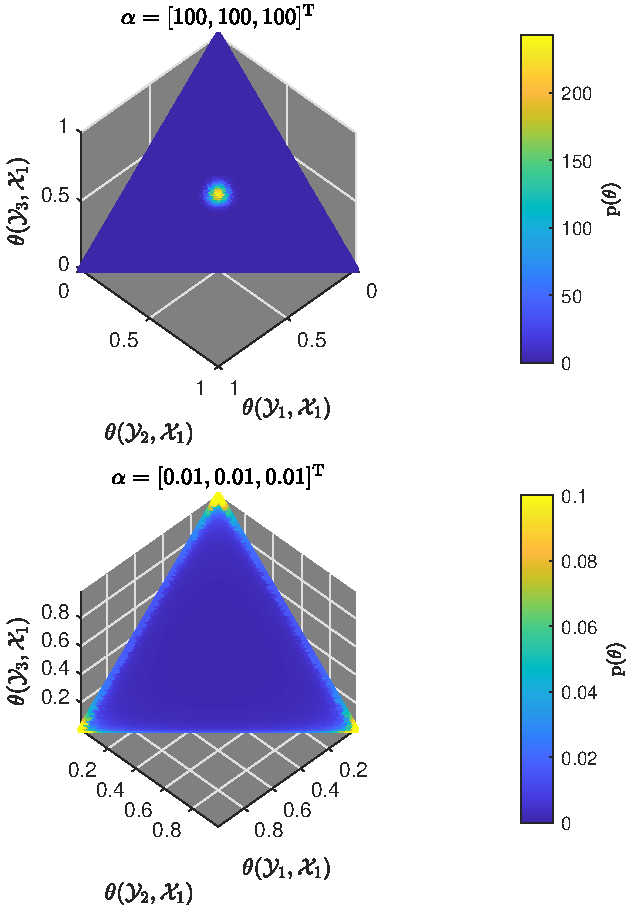
\includegraphics[width=1\linewidth]{P_theta.pdf}
\caption{Model prior PDF $\prm(\uptheta)$ for different concentrations $\alpha_0$}
\label{fig:P_theta}
\end{figure}





\subsubsection{Aggregation Properties}

As $\xrm$ is observable and $\yrm$ is not, the marginal distribution $\uptheta'$ over the set $\Xcal$, defined as $\uptheta'(x) \equiv \sum_{y \in \Ycal} \uptheta(y,x)$, will also be of interest. By the aggregation property \cite{ferguson}, $\uptheta'$ is a Dirichlet random process parameterized by $\alpha'$, where $\alpha'(x) \equiv \sum_{y \in \Ycal} \alpha(y,x)$. 

Also of interest is the joint distribution of the normalized functions $\tilde{\uptheta}(\cdot;x) \equiv \uptheta(\cdot,x) / \uptheta'(x)$ conditioned on the aggregation $\uptheta'$. It can be shown that the conditional PDF is
\begin{IEEEeqnarray}{rCl}
\prm\big( \tilde{\uptheta} | \uptheta' \big) & = & \prod_{x \in \Xcal} \Bigg[ \beta\big( \alpha(\cdot,x) \big)^{-1} \prod_{y \in \Ycal} \tilde{\uptheta}(y;x)^{\alpha(y,x)-1} \Bigg] \;,
\end{IEEEeqnarray}
a product of Dirichlet distributions defined for $\tilde{\theta} \in \left\{ \tilde{\theta}(\cdot,x) \in \Pcal(\Ycal), \quad \forall x \in \Xcal \right\}$. As shown, the normalized functions $\tilde{\uptheta}(\cdot;x)$ are independent of one another and of the aggregation $\uptheta'$. Note that $\Prm(\yrm | \xrm,\uptheta) \equiv \tilde{\uptheta}(\yrm;\xrm)$. 








\subsection{Training Set conditional PMF, $\Prm(\Drm | \uptheta)$}

Next, properties of the conditional distribution $\Prm(\Drm | \uptheta)$ will be discussed. The distribution of $\Drm$ conditioned on the model can be formulated as
\begin{IEEEeqnarray}{rCl}
\Prm\big( \Drm | \uptheta \big) & = & \prod_{y \in \Ycal} \prod_{x \in \Xcal} \uptheta(y,x)^{\bar{N}(y,x;\Drm)} \;,
\end{IEEEeqnarray}
where the dependency on the training data $\Drm$ is expressed though a transform function $\bar{N} : \Dcal \mapsto \bar{\Ncal}$, defined as
\begin{IEEEeqnarray}{rCl}
\bar{N}(y,x;D) & = & \sum_{n=1}^N \delta \left[ y,Y_n \right] \delta \left[ x,X_n \right] \;,
\end{IEEEeqnarray}
which counts the number of occurences of the pair $(y,x)$ in the training set $D$. The range of the transform is the function space 
\begin{IEEEeqnarray}{rCl}
\bar{\Ncal} & = & \left\{ \bar{n} \in {\Zbb_{\geq 0}}^{\Ycal \times \Xcal}: \sum_{y \in \Ycal} \sum_{x \in \Xcal} \bar{n}(y,x) = N \right\} \;.
\end{IEEEeqnarray}

Note that $\Prm(\Drm | \uptheta)$ depends on the training data $\Drm$ only through the transform $\bar{N}$; consequently, $\bar{N}(\Drm)$ will be a sufficient statistic for any distributions conditioned on $\Drm$. As such, it is useful to define a new random process $\nbarrm \equiv \bar{N}(\Drm) \in \bar{\Ncal}$. 

Conditioned on the model $\uptheta$, the PMF of $\nbarrm$ is a multinomial distribution
\begin{IEEEeqnarray}{rCl}
\Prm(\nbarrm | \uptheta) & = & \sum_{D : \bar{N}(D) = \nbarrm} \Prm_{\Drm | \uptheta}(D | \uptheta) \\
& = & \big|\{ D : \bar{N}(D) = \nbarrm \}\big| \prod_{y \in \Ycal} \prod_{x \in \Xcal} \uptheta(y,x)^{\bar{\nrm}(y,x)} \nonumber \\
& = & \Mcal(\nbarrm) \prod_{y \in \Ycal} \prod_{x \in \Xcal} \uptheta(y,x)^{\bar{\nrm}(y,x)} \nonumber \;,
\end{IEEEeqnarray}
where the multinomial operator $\Mcal$ is used. The mean and covariance functions of this multinomial distribution are \cite{theodoridis-ML}
\begin{IEEEeqnarray}{rCl}
\mu_{\bar{\nrm} | \uptheta}(y,x) & = & \Erm_{\bar{\nrm} | \uptheta}\big[ \bar{\nrm}(y,x) \big] = N \uptheta(y,x)
\end{IEEEeqnarray}
and
\begin{IEEEeqnarray}{L}
\Sigma_{\nbarrm | \uptheta}(y,x,y',x')  \\
\quad = N \big( \uptheta(y,x) \delta[y,y'] \delta[x,x'] - \uptheta(y,x) \uptheta(y',x') \big) \nonumber \;.
\end{IEEEeqnarray}







\subsubsection{Aggregation Properties}

As performed for the model $\uptheta$, a characterization of the function $\nbarrm$ integrated over the set $\Ycal$ will be found. Introduce the function $N' : \Dcal \to \Ncal'$, defined as
\begin{IEEEeqnarray}{rCl}
N'(x;D) & = & \sum_{y \in \Ycal} \bar{N}(y,x;D) = \sum_{n=1}^N \delta\big[ x,X_n \big]
\end{IEEEeqnarray}
where 
\begin{IEEEeqnarray}{rCl}
\Ncal' & = & \left\{ n' \in {\Zbb_{\geq 0}}^{\Xcal}: \sum_{x \in \Xcal} n'(x) = N \right\} \;.
\end{IEEEeqnarray}
Define the ``marginalized'' random process $\nrm'$ over the set $\Xcal$, defined as $\nrm'(x) \equiv \sum_{y \in \Ycal} \nbarrm(y,x) \equiv N'(\Drm)$. 


By the aggregation property of Multinomial random processes \cite{johnson}, the aggregation conditioned on the model $\uptheta$ is distributed as $\nrm' | \uptheta \sim \Mult(N,\uptheta')$. 

Also of interest is the distribution of $\nbarrm$ conditioned on its aggregation $\nrm'$. It can be shown that when conditioned on the model $\uptheta$ as well, the PMF for $\nbarrm$ is
\begin{IEEEeqnarray}{rCl}
\Prm(\bar{\nrm} | \nrm' , \uptheta) & = & \prod_{x \in \Xcal} \Bigg[ \Mcal\big( \bar{\nrm}(\cdot,x) \big) \prod_{y \in \Ycal} \left(\frac{\uptheta(y,x)}{\uptheta'(x)}\right)^{\bar{\nrm}(y,x)} \Bigg] \;,
\end{IEEEeqnarray}
which has support $\bar{\nrm} \in \left\{ {\Zbb_{\geq 0}}^{\Ycal \times \Xcal} : \sum_{y \in \Ycal} \bar{n}(y,x) = \nrm'(x), \quad \forall x \in \Xcal \right\}$. Observe that conditioning on the aggregation renders the function segments $\nbarrm(\cdot,x)$ independent of one another and that they are also Multinomial, such that $\nbarrm(\cdot,x) | \nrm'(x),\uptheta \sim \Mult\big( \nrm'(x),\uptheta(\cdot,x) / \uptheta'(x) \big)$.









\subsection{Predictive PMF, $\Prm(\yrm | \xrm,\Drm)$}

Finally, the Bayesian predicitive PMF $\Prm(\yrm | \xrm,\Drm)$ is provided. First observe that since $\Prm(\Drm | \uptheta)$ is of exponential form, the Dirichlet prior $\prm(\uptheta)$ is its conjugate prior \cite{theodoridis-ML}; thus, the model posterior PDF given the training data is
\begin{IEEEeqnarray}{rCl}
\prm(\uptheta | \Drm) & = & \frac{\Prm(\Drm | \uptheta) \prm(\uptheta)}{\Prm(\Drm)} \\
& = & \beta \left( \alpha + \bar{N}(\Drm) \right)^{-1} \prod_{y \in \Ycal} \prod_{x \in \Xcal} 
\uptheta(y,x)^{\alpha(y,x) + \bar{N}(y,x;\Drm) - 1} \nonumber \;, 
\end{IEEEeqnarray}
a Dirichlet distribution with parameter function $\alpha + \bar{N}(\Drm)$.

The concentration parameter increases proportionately with increasing volumes of training data; thus as $N \to \infty$, the posterior converges to $\prm(\uptheta | \Drm) \to \delta\big( \uptheta - \bar{N}(\Drm) / N \big)$. As more data is collected, the model can be more positively identified and used to formulate minimum risk decisions. Conversely, as $\alpha_0 \to \infty$, the prior model certainty is stronger and the posterior trends toward $\prm(\uptheta | \Drm) \to \delta( \uptheta - \alpha / \alpha_0)$, independent of the training data.

Figure \ref{fig:P_theta_D} shows the influence of the training data on the model distribution; after conditioning on the training data (via $\nbarrm$), the PDF concentration shifts away from the models favored by the prior knowledge and towards other models that better account for the observations.

\begin{figure}
\centering
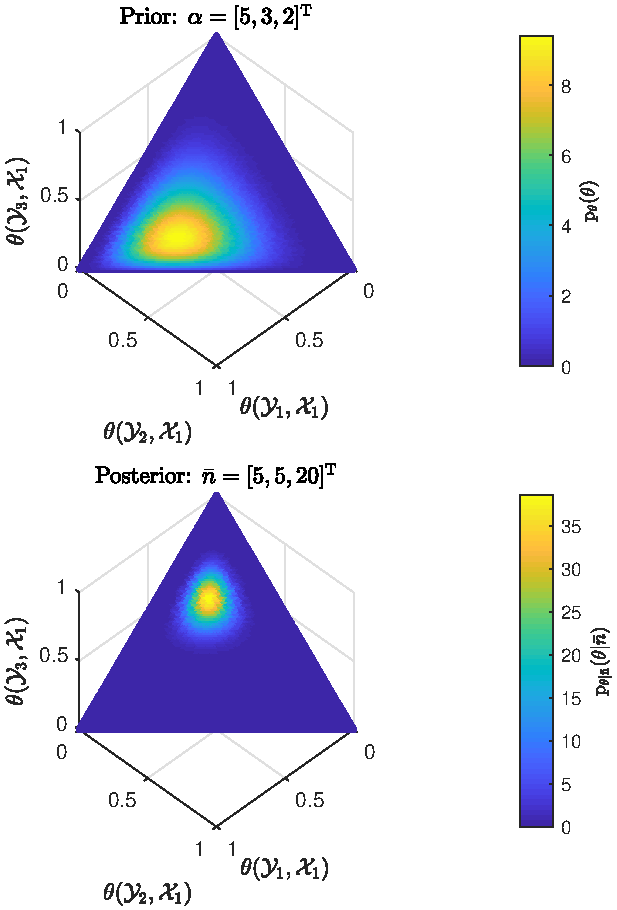
\includegraphics[width=1\linewidth]{P_theta_post.pdf}
\caption{Model $\uptheta$ PDF, prior and posterior}
\label{fig:P_theta_D}
\end{figure}


The joint PMF of $\yrm$ and $\xrm$ conditioned on the training data is expressed as \cite{murphy}
\begin{IEEEeqnarray}{rCl}
\Prm(\yrm,\xrm | \Drm) & = & \frac{\Erm_{\uptheta}\big[ \uptheta(\yrm,\xrm) \Prm(\Drm | \uptheta) \big]}{\Prm(\Drm)} = \mu_{\uptheta | \Drm}(\yrm,\xrm) \\
& = & \left(\frac{\alpha_0}{\alpha_0 + N}\right) \frac{\alpha(\yrm,\xrm)}{\alpha_0} + \left(\frac{N}{\alpha_0 + N}\right) \frac{\bar{N}(\yrm,\xrm;\Drm)}{N} \nonumber \;.
\end{IEEEeqnarray}
This is a mixture distribution between the prior expectation $\Erm[\uptheta] = \alpha/\alpha_0$ and the empirical distribution $\bar{N}(\Drm)/N$. The more subjective the model prior (i.e. larger $\alpha_0$), the more the prior mean is favored; the more data, the more the empirical PMF is favored. The marginal distribution for $\xrm$ given $\Drm$ is
\begin{IEEEeqnarray}{rCl}
\Prm(\xrm | \Drm) & = & \left(\frac{\alpha_0}{\alpha_0 + N}\right) \frac{\alpha'(\xrm)}{\alpha_0} + \left(\frac{N}{\alpha_0 + N}\right) \frac{N'(\xrm;\Drm)}{N} \;.
\end{IEEEeqnarray}

Finally, the distribution of interest is generated via Bayes rule as
\begin{IEEEeqnarray}{rCl}
\Prm(\yrm | \xrm,\Drm) & = & \frac{\Prm(\yrm,\xrm | \Drm)}{\Prm(\xrm | \Drm)} = \frac{\alpha(\yrm,\xrm) + \bar{N}(\yrm,\xrm;\Drm)}{\alpha'(\xrm) + N'(\xrm;\Drm)} \\
& = & \left(\frac{\alpha'(\xrm)}{\alpha'(\xrm) + N'(\xrm;\Drm)}\right) \frac{\alpha(\yrm,\xrm)}{\alpha'(\xrm)} \nonumber \\
&& \quad + \left(\frac{N'(\xrm;\Drm)}{\alpha'(\xrm) + N'(\xrm;\Drm)}\right) \frac{\bar{N}(\yrm,\xrm;\Drm)}{N'(\xrm;\Drm)} \nonumber \;.
\end{IEEEeqnarray}
The last representation views the distribution as a convex combination of two conditional distributions. The first distribution $\Prm(\yrm | \xrm) = \alpha(\yrm,\xrm) / \alpha'(\xrm)$ is independent of the training data and based on the prior knowledge implied via the model PDF parameter; the second distribution is the conditional empirical PMF and depends on $\Drm$, not on $\alpha$. For both, only those values $\alpha$ and $\Drm$ corresponding to the observed value $\xrm$ influence the distribution. 

The weighting factors are dependent on these values as well. For $N'(\xrm;\Drm) = 0$ or as $\alpha_0 \to \infty$, the PMF trends toward the conditional distribution $\Prm(\yrm|\xrm)$, which only depends on the model parameter $\alpha$. As the number of training examples increases or as $\alpha_0 \to 0$, $\Prm(\yrm | \xrm,\Drm)$ trends towards the empirical conditional distribution. 









\section{Density Estimation Perspective}

PGR: plot error vs N for diff a0?

This section compares the Bayesian predictive distribution $\Prm(\yrm | \xrm,\Drm)$ to the unobserved predictive PMF $\Prm(\yrm | \xrm,\uptheta)$ and investigates the effects of subjective prior knowledge. As $\bar{N}(\Drm)$ is a sufficient statistic for the training data, any distributions dependent on $\Drm$ will be replaced by their corresponding distributions of $\nbarrm$, simplifying the analysis.

For a given $\xrm$ and corresponding number of training samples $\nrm'(\xrm)$, the expected value of the estimate condtioned on the true model $\uptheta$ is
\begin{IEEEeqnarray}{L}
\Erm_{\nbarrm | \nrm',\uptheta}\big[ \Prm_{\yrm | \xrm,\nbarrm}(y | \xrm,\nbarrm) \big] \\ 
\quad = \left(\frac{\alpha'(\xrm)}{\alpha'(\xrm) + \nrm'(\xrm)}\right) \frac{\alpha(y,\xrm)}{\alpha'(\xrm)} + \left(\frac{\nrm'(\xrm)}{\alpha'(\xrm) + \nrm'(\xrm)}\right) \frac{\uptheta(y,\xrm)}{\uptheta'(\xrm)} \nonumber \;,
\end{IEEEeqnarray}
where the properties of a multinomial distribution conditioned on its aggregation have been used. The result is a convex combination of the conditional data-independent distribution $\alpha(\cdot,x) / \alpha'(x)$ and the true conditional distribution $\uptheta(\cdot,x) / \uptheta'(x)$. The convex coefficients are dependent on the ``marginal'' values $\alpha'$ and $\nrm'$; note that as the number of matching training samples $\nrm'(x)$ increases relative to $\alpha'(x)$, the estimate trends towards the true conditional PMF. 

PGR: suppress delta dependency on nbar and theta?

To aid characterization of the predictive PMF estimator, define the random process $\Delta(\cdot;\xrm,\nbarrm) \equiv \Prm_{\yrm | \xrm,\nbarrm}(\cdot | \xrm,\nbarrm) - \Prm_{\yrm | \xrm,\uptheta}(\cdot | \xrm,\uptheta)$. For a given $\xrm$ and corresponding number of training samples $\nrm'(\xrm)$, the bias of the conditional PMF estimate is
\begin{IEEEeqnarray}{rCl}
\mathrm{Bias}(y;\xrm,\nrm') & = & \Erm_{\nbarrm | \nrm',\uptheta}\big[ \Delta(y;\xrm,\nbarrm) \big] \\
& = & \frac{\alpha'(\xrm)}{\alpha'(\xrm) + \nrm'(\xrm)} \left( \frac{\alpha(y,\xrm)}{\alpha'(\xrm)} - \frac{\uptheta(y,\xrm)}{\uptheta'(\xrm)} \right) \nonumber 
\end{IEEEeqnarray}
and its covariance function is 
\begin{IEEEeqnarray}{L}
\mathrm{Var}(y,y';\xrm,\nrm') = \Crm_{\nbarrm | \nrm',\uptheta} \big[\Prm_{\yrm | \xrm,\nbarrm}(\cdot | \xrm,\nbarrm) \big](y,y') \\
\quad = \frac{\nrm'(\xrm)}{\big( \alpha'(\xrm) + \nrm'(\xrm) \big)^2} \left( \frac{\uptheta(y,\xrm)}{\uptheta'(\xrm)} \delta[y,y'] - \frac{\uptheta(y,\xrm)}{\uptheta'(\xrm)} \frac{\uptheta(y',\xrm)}{\uptheta'(\xrm)} \right) \nonumber \;,
\end{IEEEeqnarray}
where the properties of multinomial random processes have been used. Note that the bias is proportionate to the difference between the true conditional model and the data-independent estimate. The scaling factor trends to zero as $\nrm'(x)/\alpha'(x) \to \infty$; as such, more subjective priors (large $\alpha'(x)$) will lead to PMF estimates that are prone to bias. Conversely, the variance of the PMF estimate decreases with increasing $\alpha'(x)$. 


Combining the estimator bias and variance, the squared difference between the estimate and the true conditional model is
\begin{IEEEeqnarray}{rCl}
\mathcal{E}(y,y' ; \xrm,\nrm') & = & \Erm_{\nbarrm | \nrm',\uptheta} \Big[ \Delta(y;\xrm,\nbarrm) \Delta(y';\xrm,\nbarrm) \Big] \\
& = & \mathrm{Bias}(y;\xrm,\nrm') \mathrm{Bias}(y';\xrm,\nrm') + \mathrm{Var}(y,y';\xrm,\nrm') \nonumber \;.
\end{IEEEeqnarray}
As $\nrm'(x) \to \infty$, this function trends to zero and thus the underlying model $\uptheta(\cdot,x) / \uptheta'(x)$ is determined precisely. A more practical case is estimation with a finite volume of training data. Specification of the Dirichlet model prior can be interpreted as providing a distribution estimate $\alpha(\cdot,x)/\alpha'(x)$ and a confidence level $\alpha'(x)$. Higher confidence reduces error due to the variance of the estimator, but increases the error due to bias between the true model and its estimate; low confidence renders the estimate unbiased, but maximizes the estimator variance. 



To exemplify how the model estimate $\Prm(\yrm | \xrm,\Drm)$ approximates $\Prm(\yrm | \xrm,\uptheta)$, consider a scenario with $|\Ycal| = 10$. The data-independent PMF $\alpha / \alpha_0$ and true model $\uptheta$ are shown in Figure \ref{fig:P_yx_error_N_0} - note the significant mismatch. 

Figures \ref{fig:P_yx_error_a0_0_1} and \ref{fig:P_yx_error_a0_10} show how the expected value and variance of the estimate (represented by the blue markers and error bars, respectively) change for different values of $\nrm'(x)$ and $\alpha'(x)$ . Each individual plot heading provides the error $\sqrt{\sum_{y \in \Ycal} \mathcal{E}(y,y ; \xrm,\nrm')}$ to assess the quality of the PMF estimate. 

Observe that for $\nrm'(x) = 1$, the high variance of the $\alpha'(x) = 0.1$ estimate (favoring the empirical PMF) renders it worse than the $\alpha_0 = 10$ estimate; in fact, the variance is so high that the error exceeds that of the data-independent estimate $\alpha(\cdot,x) / \alpha'(x)$ (Figure \ref{fig:P_yx_error_N_0}). Conversely, for $\nrm'(x) = 10$, the confidence of the $\alpha'(x) = 10$ estimate leads to high bias and the $\alpha'(x) = 0.1$ estimate is superior. For $\nrm'(x) = 100$, both the $\alpha'(x) = 0.1$ and $\alpha'(x) = 10$ estimates begin converging to the true predictive distribution - this is guaranteed due to the full support of the Dirichlet prior.


\begin{figure}
\centering
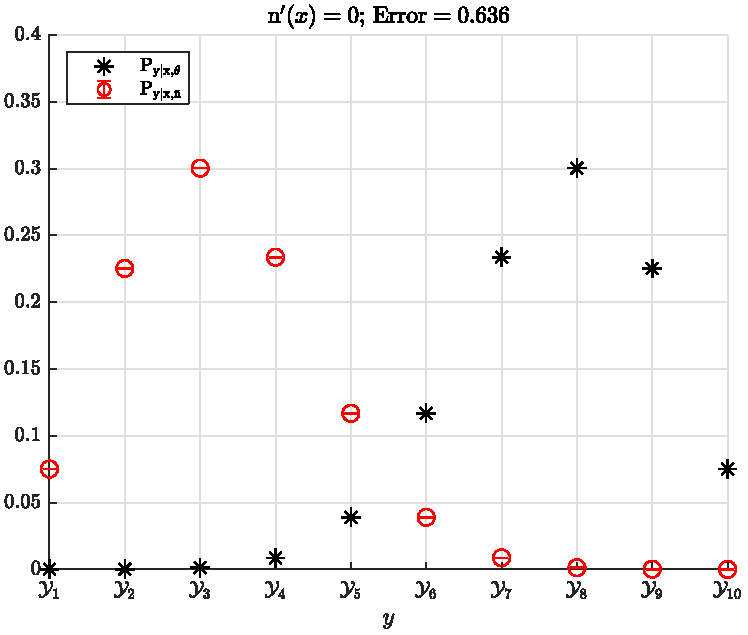
\includegraphics[width=1\linewidth]{P_yx_error_N_0.pdf}
\caption{Model $\uptheta$ estimate, no training data}
\label{fig:P_yx_error_N_0}
\end{figure}

\begin{figure}
\centering
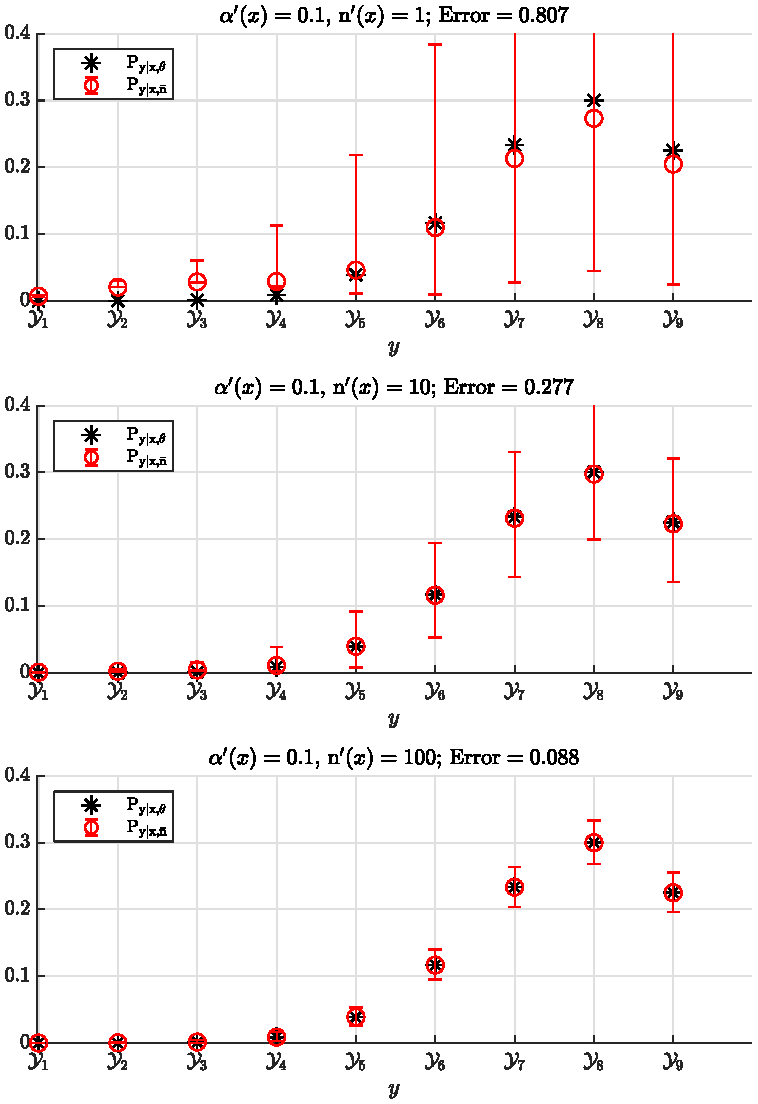
\includegraphics[width=1\linewidth]{P_yx_error_a0_0_1.pdf}
\caption{Model $\uptheta$ estimates, $\alpha_0 = 0.1$}
\label{fig:P_yx_error_a0_0_1}
\end{figure}

\begin{figure}
\centering
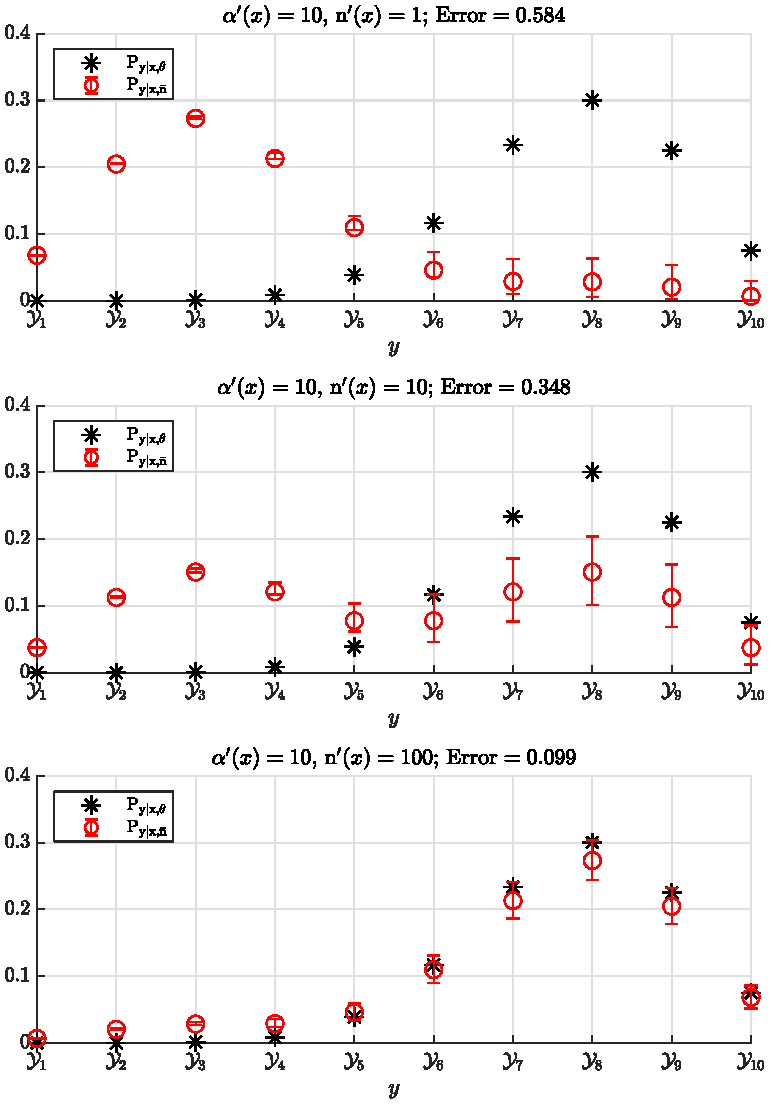
\includegraphics[width=1\linewidth]{P_yx_error_a0_10.pdf}
\caption{Model $\uptheta$ estimates, $\alpha_0 = 10$}
\label{fig:P_yx_error_a0_10}
\end{figure}





\section{Conclusions}

This article has shown how a Dirichlet prior distribution may be used for a Bayesian approach to machine learning prediction. An analysis of how well the Bayesian predictive distributions match the true predictive distributions has been performed for a variety of different non-informative and subjective priors.

The conditional second moments of the difference between the two predicitve PMF's have important applications for Bayesian regression, specifically for determining the expected squared-error loss. This will be a primary focus of future work.





















\bibliographystyle{plain}
\bibliography{{../References/phd_bib}}

\end{document}


























